% !TEX encoding = UTF-8 Unicode
\chapter*{Introduction}         % ne pas numéroter
\label{chap-introduction}       % étiquette pour renvois
\phantomsection\addcontentsline{toc}{chapter}{\nameref{chap-introduction}} % inclure dans TdM

% Note: This is an un-numbered chapter.

Grinding is a particle size reduction process used in the mineral processing industry to liberate valuable minerals from ore as part of the concentration process. Figure \ref{fig:process-block-diagram} shows the steps in a typical copper concentration process.
\begin{figure}[htp]
	\centering
	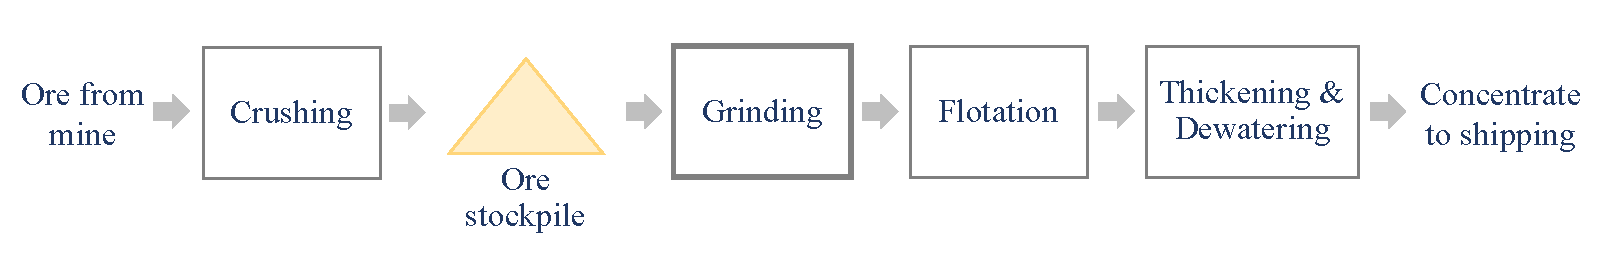
\includegraphics[width=15.5cm]{images/process_block_diagram.pdf}
	\caption{Processing steps in a copper concentrator} \label{fig:process-block-diagram}
\end{figure}

%TODO: JB suggested more introduction to grinding circuits and a diagram:
%I think you miss a description of the process:- grinding machines- physical breakage- typical circuit you'll be focussing on: SAG mill
% Doesn't have to be very long, but you could probably have a few paragraphes and a couple of figures.
Grinding is essentially the fracturing of rock particles, which can be achieved by the application of large compressive forces, especially when these forces are applied rapidly, such as during high-speed impacts. The extent to which ore particles are resistant to fracture depends on complex properties of the ore, such as the presence of micro and macro flaws in the structure of the material. This is the main reason why ore properties have a significant effect on the grinding process.

Tumbling mills are the most common type of grinding equipment used in hard rock grinding applications. In tumbling mills, ore particles are fractured by various breakage mechanisms including impact breakage, abrasion, and attrition \citep{king_chapter_2012}. The two main types of tumbling mills are the \gls{SAG} mill and the ball mill. The \gls{SAG} mill, which is the focus of this research, is used for primary grinding of the \textit{run-of-mine} ore which comes from the mine after crushing. In a \gls{SAG} mill, large ore particles play a role in the grinding process as well as grinding media (steel balls) added by the operator. One or more ball mills are typically used in a second stage of grinding to grind oversize particles from the discharge of the \gls{SAG} mill circuit. Figure \ref{fig:sag-ball-circuit-diag} is a simplified diagram of a typical SAG-and-ball-mill circuit.%
\begin{figure}[htp]
	\centering
	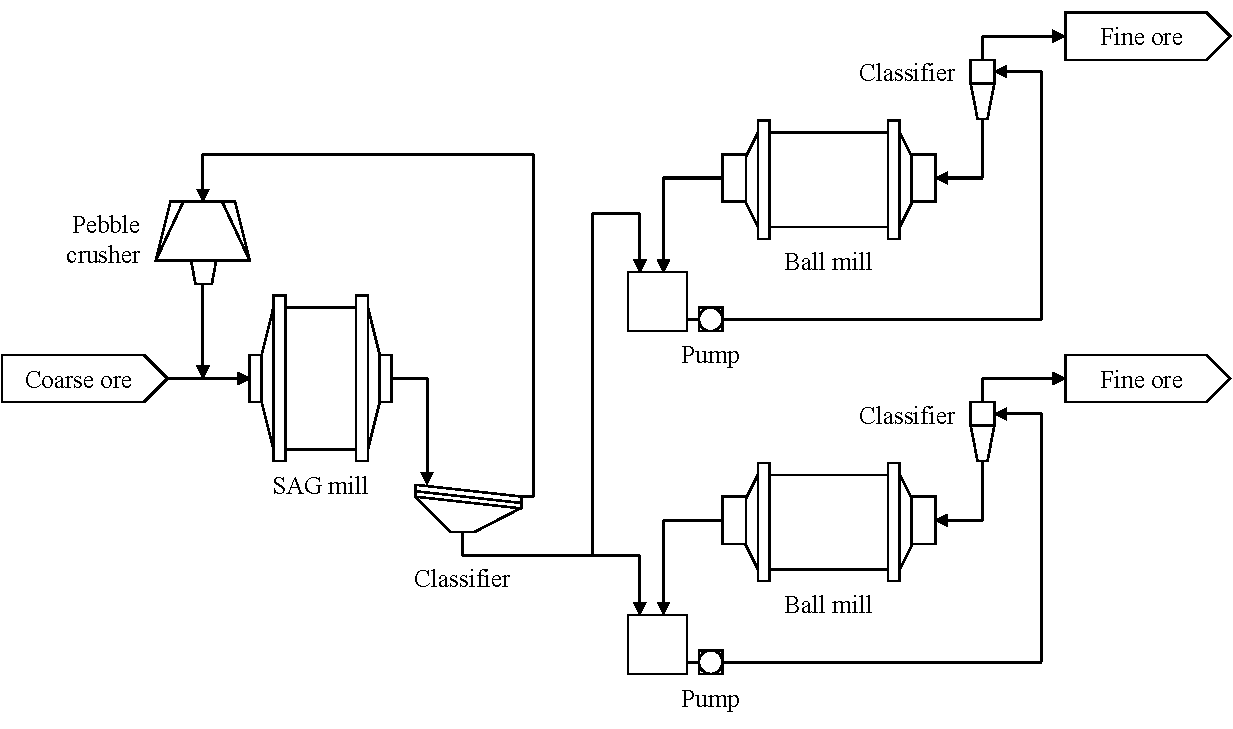
\includegraphics[width=14cm]{images/sag-ball-circuit-diag.pdf}
	\caption{Typical SAG and ball mill circuit arrangement} \label{fig:sag-ball-circuit-diag}
\end{figure}

Effective control and optimization of SAG mill circuits is challenging for a number of reasons---large variations in the properties of the ore feed material, multiple strongly-coupled interacting variables, long time delays, non-linear and time-varying input-output characteristics, process variables that are difficult to measure, and difficulties in identifying process models of actual operations \citep{olivier_dual_2012, gough_sag_2015, le_roux_throughput_2016, aguila-camacho_control_2017}. 

Any input that has a material effect on the state or behaviour of a process and is not manipulated by the control system is defined as a disturbance. Changes in the properties of the ore feed are a significant problem because they are difficult to measure accurately in real time and their impact on the grinding process and control system can be severe \citep{herbst_optimal_1988, garrido_multivariable_2009, remes_grinding_2010, liu_development_2018}. \cite{powell_applying_2009} summarized the effects of variations in ore properties as a chain reaction:

Variable ore $\to$ variable operation $\to$ variable grind $\to$ variable recovery $\to$ lower recovery. 

One of the primary goals of industrial process control is to maintain desired performance in the presence of unmeasured disturbances \citep{astrom_computer_1997}. By detecting and correcting errors in the estimates of the process outputs or states, feedback control systems are able to attenuate the effects of disturbances and thus reduce variation in process variables. This is known as the regulation problem and is common in industrial process control applications where the goal is to maintain stationary operating conditions as closely as possible.

The main benefit of effective regulation is that the process variables remain close to the desired set points. This is particularly important when there are operating constraints on critical variables that limit the overall process performance. For example, the power output capacity of an electric motor must not be exceeded for safety reasons. In such cases, it may not be possible to reject a disturbance completely. Some variations in the output variables may be unavoidable and thus, ore feed disturbances can have knock-on effects on the downstream process operations (i.e. the separation process). By reducing the magnitude of variability caused by disturbances, the process may be operated closer to the operating constraints on average, yielding a higher performance than would be achievable with high variability, and reducing the magnitude of variations transmitted to downstream processes.

\subsection*{Motivation}

The motivation for this work is to improve grinding process control design through the use of better models of process disturbances. Good simulation models are required to develop and test control systems, including methods to simulate the characteristics of the disturbances that exist in real operations as closely as possible. As well as enabling more realistic grinding process simulations, disturbance models based on a more sophisticated understanding and characterization of disturbances could be used, directly or indirectly, in the design of model-based observers and controllers. Therefore, there is a need for a variety of versatile disturbance models, and methods with which to incorporate them into control strategies.

%A better understanding of ore variability could also be useful in identifying process improvements in the mining operation, although that is not the primary motivation of this work.

\section*{Background and objectives}

The work is part of a three-year research and development project by the \textit{Laboratoire d’observation et d’optimisation des procédés} (LOOP) at \textit{Universit\'e Laval}, with financial support from the Government of Qu\'ebec and Nemaska Lithium Corporation. The overall goal of the project is to determine the extent to which technological innovations could transform the current paradigm of mineral processing which is energy intensive and results in significant greenhouse gas emissions. The project consists of two main initiatives:

\begin{enumerate}
	\item development of dynamic operating models of production units,
	\item development of circuit configurations, process controls, and real time optimization strategies.
\end{enumerate}

Aligned with the second initiative, the specific goals of this work are to identify or develop disturbance models and observers specifically tailored to the types of disturbances that exist in grinding operations.

\section*{Organisation of this thesis}

Chapter \ref{chap-lit-review} contains a review of the related academic literature and statements of the objectives and contributions of this research. Chapter \ref{chap-methods} describes the methods used in the work, including disturbance models, observer designs, and the grinding simulation model used to evaluate the observers. Chapter \ref{chap-simulation} describes the simulations carried out to demonstrate the disturbance models and to evaluate the performance of various observer designs.
% Removed
%Chapter \ref{chap-identification} describes numerical experiments to investigate potential methods of identifying disturbance models from data.
